% !TeX spellcheck = de-de

\documentclass{beamer}

\usetheme{Warsaw}             % Falls Ihnen das Layout nicht gef�llt, k�nnen Sie hier
                              % auch andere Themes w�hlen. Ein Verzeichnis der m�glichen 
                              % Themes finden Sie im Kapitel 15 des beameruserguide.


\setbeamertemplate{footline}[frame number] %Seitenzahlen

\usepackage[utf8]{inputenc} % um Umlaute direkt eingeben zu
\usepackage[german]{babel}
\usepackage{amsmath}
\usepackage{amsfonts}
\usepackage{amssymb}
\usepackage{graphicx}
\usepackage{tikz}
\usepackage{stmaryrd} % for llbracket
\usepackage{algorithm} %for algorithms
\usepackage{algpseudocode} %for algorithms
%\usepackage{caption}
\usepackage{subcaption} %for subfigure
\usepackage[3D]{movie15} %for interactve 3d plot 

\usepackage{wrapfig} % for using wrapfigure

\usepackage{bigdelim}
\usepackage{caption}
\usepackage{subcaption}
\usepackage{ltxtable}
\usepackage{float}
%\usepackage{pgfplotstable, booktabs} %to generate tables from data files
\usepackage{cancel} %um durchzustreichen


\usepackage{bibunits} %to split bibliography

\usepackage{../Arbeit/makros}
\usepackage{todo}

\makeatletter
% Detect mode. mathpalette is used to detect the used math style
\newcommand<>\Alt[2]{%
    \begingroup
    \ifmmode
        \expandafter\mathpalette
        \expandafter\math@Alt
    \else
        \expandafter\make@Alt
    \fi
    {{#1}{#2}{#3}}%
    \endgroup
}

% Un-brace the second argument (required because \mathpalette reads the three arguments as one
\newcommand\math@Alt[2]{\math@@Alt{#1}#2}

% Set the two arguments in boxes. The math style is given by #1. \m@th sets \mathsurround to 0.
\newcommand\math@@Alt[3]{%
    \setbox\z@ \hbox{$\m@th #1{#2}$}%
    \setbox\@ne\hbox{$\m@th #1{#3}$}%
    \@Alt
}

% Un-brace the argument
\newcommand\make@Alt[1]{\make@@Alt#1}

% Set the two arguments into normal boxes
\newcommand\make@@Alt[2]{%
    \sbox\z@ {#1}%
    \sbox\@ne{#2}%
    \@Alt
}

% Place one of the two boxes using \rlap and place a \phantom box with the maximum of the two boxes
\newcommand\@Alt[1]{%
    \alt#1%
        {\rlap{\usebox0}}%
        {\rlap{\usebox1}}%
    \setbox\tw@\null
    \ht\tw@\ifnum\ht\z@>\ht\@ne\ht\z@\else\ht\@ne\fi
    \dp\tw@\ifnum\dp\z@>\dp\@ne\dp\z@\else\dp\@ne\fi
    \wd\tw@\ifnum\wd\z@>\wd\@ne\wd\z@\else\wd\@ne\fi
    \box\tw@
}

\makeatother



\AtBeginSection[]{\frame<beamer>{\frametitle{Content} \tableofcontents[current]}}

%\titlehead{
\includegraphics[height=0.5cm]{../Arbeit/rwth.pdf} \hspace{1cm}
%
\includegraphics[height=0.5cm]{../Arbeit/IGPM_logo_klein.png}
%}

\subject{Master Thesis}
\title{Discontinuous Galerkin Methods for the \MA Equation}
\subtitle{\Large Discontinuous Galerkin Verfahren zur Lösung der Monge-Amp\`ere-Gleichung}
\author{Elisa Friebel} %\\ Matrikelnummer: 295932
\date{\today}
%\publishers{Gutachter: Prof. Dr. rer. nat. W. Dahmen\\ Prof. Dr. rer. nat. S. Noelle}
\date{20. Januar 2015 \\[.5\baselineskip] Mastervortrag}

\begin{document}
\frame{\maketitle}

\begin{bibunit}[plain]

\section{\MA Gleichung}

\begin{frame}{Die \MA Gleichung}
\begin{block}{\MA (MA) Gleichung mit Dirichlet-Randdaten}
 \begin{align*}
	 \mydet{D^2 u} &= f \textnormal{ in } \Omega \\ %\label{eq: MA eq}\\
	 u & = g \textnormal{ on } \partial \Omega, %\label{eq: MA equation dirilecht} 
 \end{align*}
 \end{block}
\pause
Anwendungsgebiete für Gleichung vom Typ \MA
\begin{itemize}
	\item Astrophysik
	\item Differentialgeometrie
	\item Wirtschaft
	\item Optimaler Transport
	\item Optik
\end{itemize} 
\end{frame}

%\subsection{Existence and Uniqueness}
\begin{frame}{Existenz von Lösungen}
	Sei $F$ der \MA Operator, d.h. $F= \detHess{u} - f$
	\begin{itemize}
		\item F ist ein nichtlinearer Operator zweiter Ordnung
		\pause
		\item $F$ ist elliptisch für strikt konvexe Funktionen $u$ und $f > 0$. %\cite{GT1983}
		\pause
		\item Existenz von klassischen Lösungen hängt von der Regularität der rechten Seite und dem Gebiet ab
		\pause
		\item klassische Lösungen sind nicht eindeutig
		\pause
		\item keine generelle schwache Formulierung\\
		 $\rightarrow $ im besonderen keine variationelle Formulierung, in der hohe Ableitungen auf Testfunktionen übertragen werden
	\end{itemize}
\end{frame}

\begin{frame}{Schwacher Lösungsbegriff}
	\begin{block}{Viskositätslösung{\cite[Definition 1.1]{FGN2013}}}
		We nennen eine strikt konvexe Funktion $u \in C^0(\Omega)$ eine \emph{Viskositäts-Unterlösung(-Überlösung)} der \MA Gleichung, falls für jeden Punkt $x_0 \in \Omega$ und Funktion $\varphi \in C^2(\Omega)$, die
		\[
		   u \leq \varphi \;(\geq \varphi) \text{ in }\Omega \text{  and  } u(x_0) = \varphi(x_0)
		\] erfüllen, es gilt, dass
		\[
			F[\varphi](x_0) \leq 0 \;(\geq 0).%\mydet{D^2 \varphi(x_0)} - f \leq 0 (\geq 0).
		\]

\end{block}
	Viskositätslösungen sind eindeutig.
	%u-\varphi hat ein maximum(minimum), d.h. DF(u-\varphi)\leq(\geq)
\end{frame}

%\subsection{Numerical Schemes}
\begin{frame}{Numersiche Verfahren}
Numerische Verfahren für die \MA Gleichung können in 4 Kategorien eingeteilt werden \cite[p.210]{FGN2013}: 
\begin{enumerate}
	\item Direkte finite Differenzen Schemata,
	\item Methoden basierend auf variationellen Prinzipien und Methoden basierend auf der Approximation unendlich-dimensionaler Räume durch endlich-dimensionaler Räume,
	\item Methoden basierend auf endlichen Basiserweiterungen und Approximieren von partiellen Differentialgleichungen an Stichprobenpunkten,
	\item Methoden, die in keiner der vorher genannten Bereiche gehören.
\end{enumerate}

\end{frame}

\begin{frame}{Finite Differenzen Schemata (FDS)}
Standard FDS (z.B. der 9-Punkte-Stern) sind uneindeutig lösbar:\\
	Lösen des nichtlinearen System mit einem Newton-Verfahren liefert verschiedene Ergebnisse für unterschiedlich gewählte Startwerte
\pause

Vorteile der FDS
\begin{itemize}
	\item Beweisrahmen für Konvergenzbeweise
	\item es existieren FDS, die bewiesen gegen die Viskositätslösung konvergieren
\end{itemize}
\begin{columns}[c]
\begin{column}{0.55\textwidth}
\pause

Nachteile der FDS
\begin{itemize}
	\item keine bewiesenen Konvergenzraten
	\item große Sterne, nicht anwendbar für viele Gebiete
	\item keine genesteten Iterationen 
\end{itemize}
\end{column}

\pause
\begin{column}{0.35\textwidth}
\begin{figure}
  \begin{center}
    
\usetikzlibrary{calc}

\newcommand{\baryc}[3]{  ($({ {#1}*\xOneRef + #2*\xTwoRef +#3*\xThreeRef}, 
                                                { {#1}*\yOneRef + #2*\yTwoRef +#3*\yThreeRef})$)  }

\begin{tikzpicture}[scale = 0.6,
]
\edef \n {4}
			
\foreach \x in  {0,...,\n}
	{
		\draw (0, \x) -- (\n, \x);
		\draw ( \x,0) -- (\x,\n);
	}

\foreach \x in  {(0,1), (1,0), (3,0), (0,3), (1,4), (4,1), (3,4), (4,3), (1,1), (1,2), (1,3), (2,1), (2,3), (3,1), (3,2), (3,3)}
	{
		\draw [thick](\n/2,\n/2) -- \x;
		\draw \x circle [radius=0.1];
	}


\end{tikzpicture}
  \end{center}
\end{figure}

\end{column}
\end{columns}
\end{frame}

\begin{frame}{Finite Element Methoden (FEM)}
Vorteil der FEM
\begin{itemize}
	\item erweiterbar auf komplexere Gebiete
	\item gut parallelisierbar
\end{itemize}
\pause
Nachteile der FEM
\begin{itemize}
	\item keine variationelle Formulierung der \MA Gleichung
	\item bisher existiert keine FEM, die bewiesen gegen Viskositätslösungen konvergiert
	\item Genestete Iterationen sind einfach zu realisieren
\end{itemize}
\end{frame}

\section{Eine Discontinuous Galerkin Methode zur Lösung der \MA Gleichung}
\subsection{Motivation}
\begin{frame}{Picard Linearisierung}
\begin{itemize}
\item Konvektionsterm: $\nabla \cdot (A(u) \nabla u )$
\item Entkoppeln der Koeffizientenmatrix $A(u)$ und $\nabla u$
\item Für $i\in \N$ wiederholtes Lösen der Gleichungen 
	\begin{align}
	\nabla \cdot (A(u^{i} )\nabla u^{i+1}) \label{eq: Picard linearisation}
	\end{align}
\item \eqref{eq: Picard linearisation} ist linear in $u^{i+1}$.
\item konvergiert langsamer als ein Newton-Verfahren, hat einen größeren Konvergenzradius
\end{itemize}
\end{frame}

\begin{frame}{Entkoppeln der MA Gleichung}
\begin{align*}
\visible<1->{	
	&\dyy u{x}  \dyy u{y}  -\dyx u {x}{y} \dyx u {y}{x} = f} \\
	\visible<2->{\Leftrightarrow \; &\mycof {D^2 u }:D^2 u  = 2f,}
\end{align*}
\visible<2->{dabei ist im zwei-dimensionalen Fall die Kofaktormatrix von $D^2 u$ definiert durch
\[
	\cofHess u := \begin{pmatrix}
		u_{xx} & - u_{xy} \\
		-u_{yx} & - u_{yy} 
	\end{pmatrix}.
\]}
\visible<3->{
Divergenz-Form
\begin{align*}
	- \nabla \cdot \left( \mycof{ D^2 u} \nabla u \right)  = -2f. 
\end{align*}
}
\end{frame}

\begin{frame}{Picard Iteration zur Lösung der MA Gleichung}
	Sei ein Startwert $u^0$ gegeben. Löse für $i \in \N$
	\begin{align}
		- \nabla \cdot \left( \cofHessH{u^i} \nabla u^{i+1} \right)  = -2f \label{eq: Picard Iteration}
	\end{align}
	\pause mithilfe des symmetrischen Interior-penalty-Galerkin (SIPG) Verfahrens

	\pause
	\begin{itemize}
		\item \eqref{eq: Picard Iteration} ist ein verallgemeinertes Poisson  Problem (GPP)\\
			\pause $\rightarrow$ d.h. linear in den zweiten Ableitungen von $u_h^{n+1}$
		\item unstetige Elemente, da $\cofHessH{u_h^n}$ unstetig ist (für Standard finite Elemente)
	\end{itemize}

\end{frame}

\subsection{Symmetrisches Interior-Penalty-Galerkin Verfahren}

\begin{frame}{Diskrete variationelle Formulierung des GPP}
Sei $\triang$ eine Triangulierung von $\Omega $ und der FE-Raum \[V_h =  \{f \in L^2(\Omega);  f|_T \in \mathcal P_k (T) \text{ for every } T \in \triang\}\] gegeben. 
\pause
			\begin{align*}
				-\myIntX \Omega {v_h \nabla \cdot (A \nabla u_h)}=
				 \myIntX \Omega {v_h f} \qquad \forall v_h \in V_h. %\label{eq: variational form}
			\end{align*}
Partielle Integration auf jeder Zelle ergibt
			\begin{align*}
				%a(v, u) = & 
				\sum_{T \in \triang} \myIntX T {\nabla v_h \cdot A \nabla u_h }
					- \sum_{T \in \triang} \myIntS  {\partial T} { v_h A \nabla u_h \cdot \mathbf n}.
			\end{align*}
\end{frame}

\begin{frame}{Herleitung des SIPG Verfahrens}
\alt
	{
		\alt{Symmetrisieren}
			{Vernachlässige den Sprung in $\nabla u$ wegen der Glattheit von $u$}<3->
	}
	{Summieren und Umschreiben mit Sprung und Mittelwert liefert}<2-> % we have
	\begin{align*}
				   \sum\limits_{T \in \triang} \myIntX  T { \nabla v_h \cdot A \nabla u_h} 
					& - \sum\limits_{e \in \edgesi}\myIntS {e} {
					\left(
					  \Alt 
					  	{\Alt 
					  		{\Alt
					  			 {\jump {u_h \average{ A \nabla v_h}}   }
					  			 {\textcolor{red}{\jump {u_h \average{ A \nabla v_h}}   }}<4->
					  		}
					         { \cancel{\jump {\average {v_h}  A \nabla u_h}}}<3->
					    }
					    {\jump {\average {v_h}  A \nabla u_h}}<2->
					 + \jump {v_h \average{ A \nabla u_h}} \right)}\\
				& - \sum\limits_{e \in \edgesb}
				         {\Alt 
				         	{ \myIntS {e} {\textcolor{red}{
				         			\left(
				         			  \textcolor{black}{v A \nabla u \cdot \mathbf n} + u_h A \nabla v_h \cdot \mathbf n
				         			\right)
  			         	     }}}
			  			    {\myIntS {e} {v_h A \nabla u_h \cdot \mathbf n}}<4->
			  			  }
	\end{align*}
	\Alt{$\Rightarrow$ Addiere den Term auch auf der rechten Seite}
	{}<4->
\end{frame}

\begin{frame}{Penalty terms to enforce continuity and Dirichlet boundary conditions}
%	\Alt{Add penalties to enforce continuity and Dirichlet boundary conditions}{}<3>
	\begin{align*}
	a(v_h,u_h) =  &\sum\limits_{T \in \triang} \myIntX  T { \nabla v_h \cdot A \nabla u_h} \\
	  & \Alt
	  		{\Alt
	  			 { -\sum\limits_{e \in \textcolor{black}{\edges}}\myIntS e { \jump {v_h \average{A \nabla u_h} }}
	  			   - \sum\limits_{e \in \textcolor{black}{\edges}}\myIntS e { \jump{ u_h \average{ A \nabla v_h}}}}
	  			 { -\sum\limits_{e \in \textcolor{red}{\edges}}\myIntS e { \jump {v_h \average{A \nabla u_h} }}
	          	  - \sum\limits_{e \in \textcolor{red}{\edges}}\myIntS e { \jump{ u_h \average{ A \nabla v_h}}}} }<3->
	  		{ -\sum\limits_{e \in \edgesi}\myIntS e { \jump {v_h \average{A \nabla u_h} }}
	 		  - \sum\limits_{e \in \edgesi}\myIntS e { \jump{ u_h \average{ A \nabla v_h}}}}<2-> \\ 
	  & \Alt
	        {
	        	\Alt
	        		{\textcolor{red}{+\sum\limits_{e \in \edges} \myIntS e { \frac \sigma {|e|} \jump {v_h} \jump {u_h}} }}
	        		{}<3->
	        }
	  		{-\sum\limits_{e \in \edgesb}\myIntS e { v_h A \nabla u_h \cdot \mathbf n} 
	    	 - \sum\limits_{e \in \edgesb}\myIntS e { u_h A \nabla v_h \cdot \mathbf n} }<2->
	 \end{align*}
	 
	 \begin{align*}
	 	l(v_h) =& \sum\limits_{T \in \triang} \myIntX  T { v_h f}
	 		 -\sum\limits_{e \in \edgesb}\myIntS e { g A \nabla v_h \cdot \mathbf n}
	 		 \uncover<3>{\textcolor{red}{+\sum\limits_{e \in \edgesb} \myIntS e {\frac \sigma {|e|} v_h g}}}
	 \end{align*}
\end{frame}

\begin{frame}{Korrektheit des SIPG Verfahrens}
Die Energie-Norm $\eNorm \cdot$ ist definiert durch
\[
	\eNorm v ^2 := \LTwonorm{\nabla v}^2 + \frac 1 \sigma \sum_{e \in \edges} |e|\LTwonormE{\average{\nabla v}}^2 + 2 \sigma \sum_{e \in \edges} \frac 1 {|e|}\LTwonormE{\jump{v}}^2\]
\pause
	\begin{itemize}
		\pause
		\item $a$ ist bilinear
		\pause
		\item $a$ ist beschränkt bzgl. der Energie-Norm $\eNorm \cdot$, falls $\sigma \geq \sigma^*$
		\pause
		\item $a$ is koerziv bzgl. der Energie-Norm $\eNorm \cdot$, falls $\sigma \geq \sigma^*$
		\pause
		\item es existiert ein eindeutiges $u \in V_h$, so dass $a(u,v) = l(v) \forall v \in V_h$
	\end{itemize}
\end{frame}

\begin{frame}{Fehlerabschätzung für SIPG}
	\begin{block}{Theorem}
		Sei $u$ die exakte Lösung des GPP und $\sigma \geq \sigma^*$, so dass $a$ stabil ist. 
		Weiterhin erfülle $u_h \in V_h$
		\[
		a(v_h, u_h) = l(v_h) \qquad \forall v_h \in V_h.
		\]
		Dann existiert eine positive Konstante $C$ unabhängig von $h$, so dass
		\[
		\eNorm{u - u_h } \leq \left(1+\frac C \alpha\right) \inf_{v_h \in V_h} \eNorm{u - v_h}.
		\]
		Hierbei ist $\alpha$ die Koerzivitätskonstante von $a$. 
	\end{block}
\end{frame}


\subsection{Herausforderungen für die Picard Iteration}
\begin{frame}{Startwert für die Picard Iteration}
%In \cite[Remark 2.1]{DG2006a} 
Es wurde gezeigt, dass eine gute Schätzung für die Lösung der MA Gleichung, die Lösung von 
\begin{align*}
	\triangle u &= \sqrt{2f} \text{ in } \Omega, \\ 
	u &= g \text{ on }\partial \Omega.
\end{align*}
ist.
\pause
Genestete Iteration
\begin{itemize}
\item auf dem gröbsten Gitter die Startfunktion $u^0_{h_1}$, e.g. $\frac 1 2 ({x_1^2} + {x_2^2}) $ 
\item auf dem Gitter $\mathcal{T}_{h_{l}}$ wird als Startwert die letzte Lösung vom vorherigen Gitter genutzt
\end{itemize}
\end{frame}

\begin{frame}{Konsistenz-Test der Picard iteration}
Simples MA Problem mit der exakten klassischen Lösung $\frac 1 2 (x_1^2 + x_2^2 )$. 
\begin{align*}
	\mydet {D^2 u} = 1 \text{ in } \Omega \quad \text{  and  }\quad 
	u = \frac 1 2 (x_1^2 + x_2^2 )\text{ on }\partial \Omega,
\end{align*}
%\vspace{-0.5cm}
\pause
Rel. $L^2$-Fehler auf einem Gitter mit $h=\frac 1 2$ und dem exakten Startwert $u_0=u$

\begin{figure}[H]
	\centering
	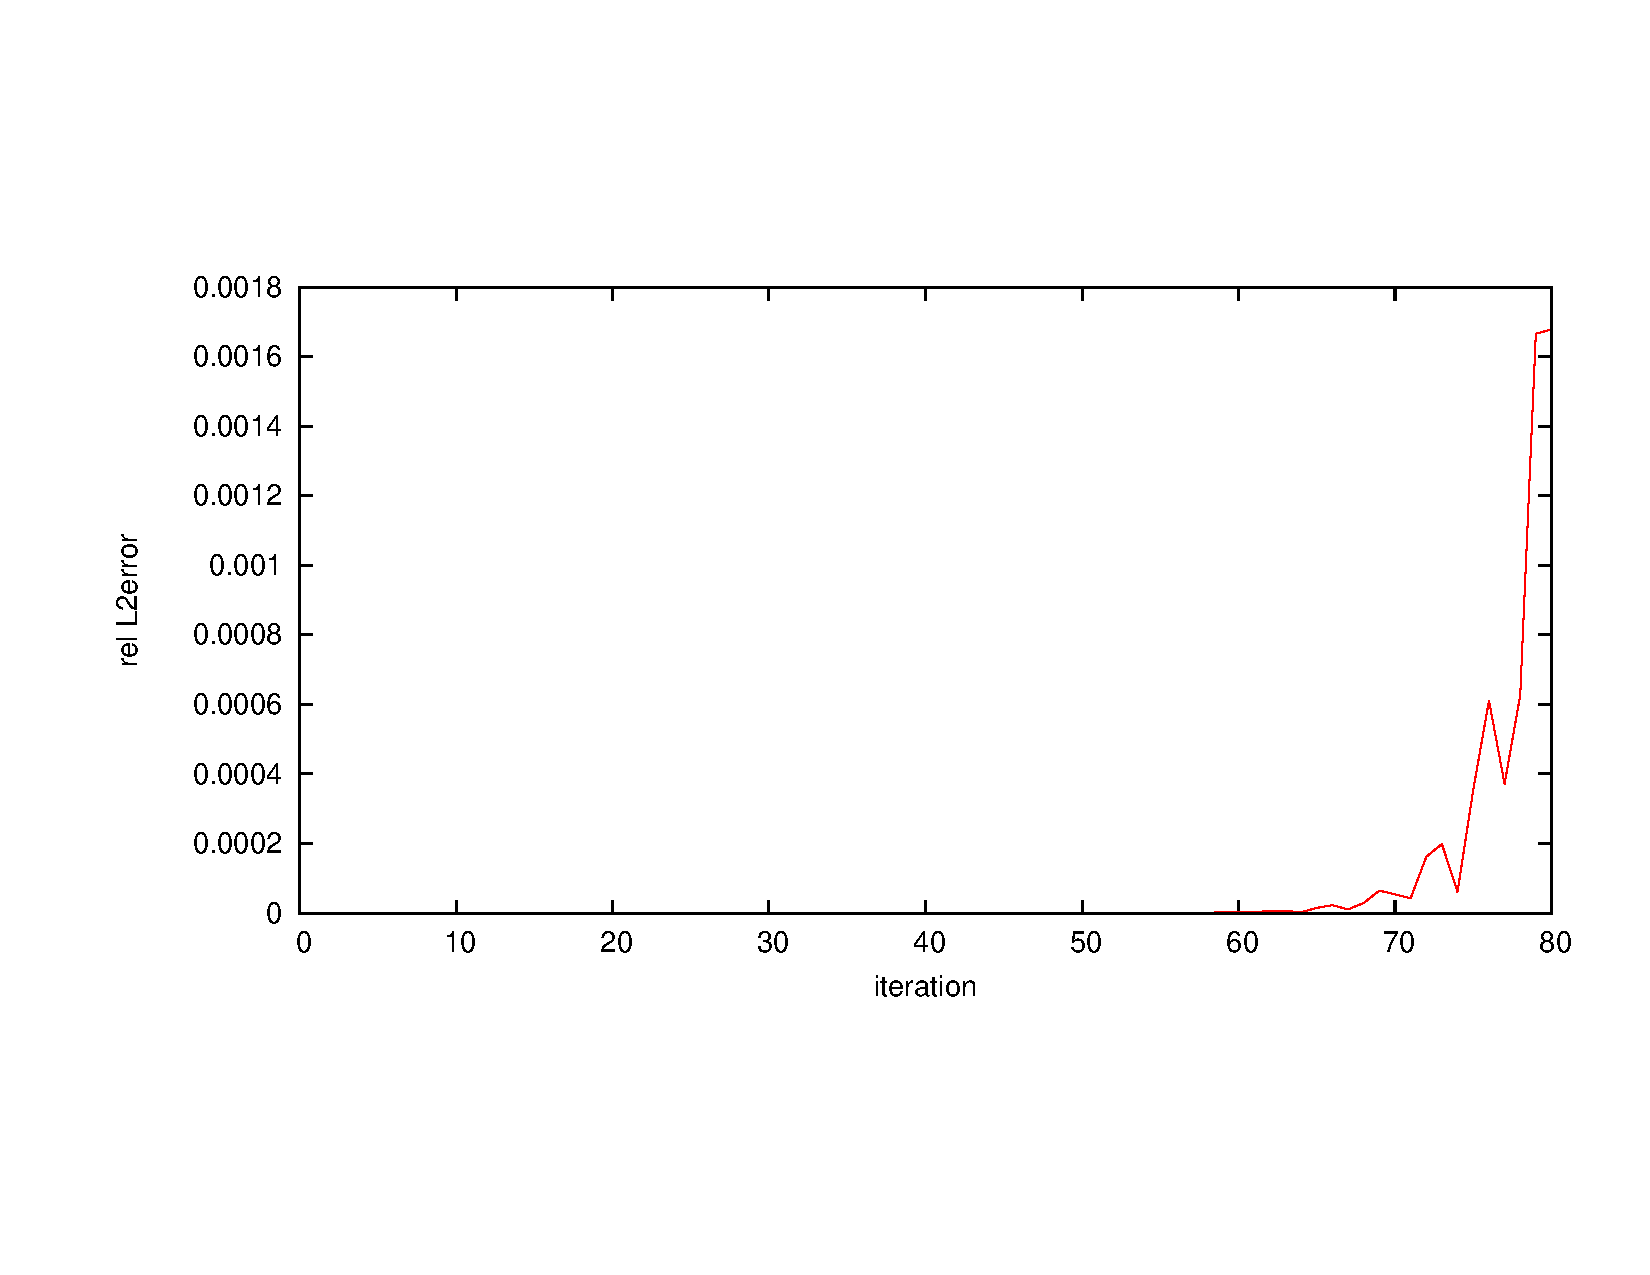
\includegraphics[trim = 2cm 4cm 1cm 4cm, scale =0.3]{../Arbeit/plots/consisctency_first_try.pdf}
	%\label{fig: consisctency_first_try}
\end{figure}
\end{frame}

\begin{frame}{Ein weiterer Penalty-parameter}
  \begin{columns}
	\begin{column}{0.9\textwidth}
%	\begin{wrapfigure}{r}{0.5\textwidth}
		\begin{figure}[H]
			\centering
			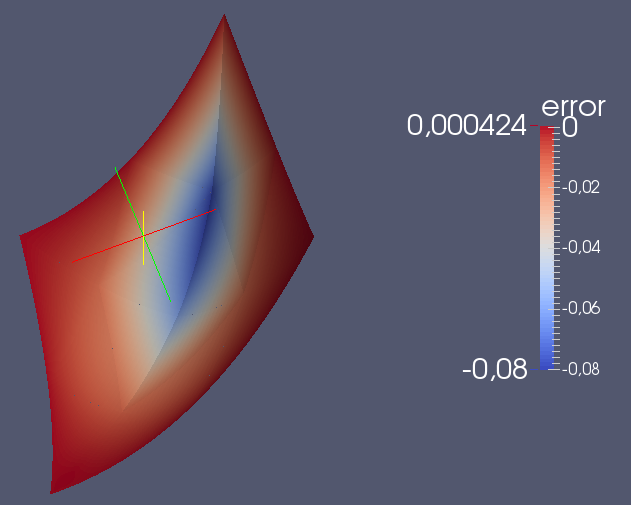
\includegraphics[width=.7\textwidth]{../Arbeit/plots/sharp_edges.png}
%			\includemovie[ 
%			 poster,controls, 
%			 label=mylabel]{5cm}{5cm}{sharp_edges.u3d} 
			\caption{Numerische Lösung}
			\label{fig: sharp edges}
%	\end{wrapfigure}
		\end{figure}
	\end{column}
	\hspace{-2cm}
	\pause
	\begin{column}{0.3\textwidth}
%		\todo{.vtu file?}
		\begin{itemize}
			\item scharfe Kanten
			\item hängt von der Triangulierung ab, obwohl die Lösung in $V_h$ enthalten
		\end{itemize}
	\end{column}
  \end{columns}
\end{frame}

\begin{frame}{Ein weiterer Penalty-parameter}
\begin{itemize}
\item mehr Regularität in der ersten Ableitung fordern
\pause
\item Neilan benutzt in seiner DG Methode für kleine Polynomgrade einen zusätzlichen Penalty-Term
\end{itemize}
\[
	\sum_{e \in \edgesi} \sigma^G |e |\myIntS e {\jump{ \nabla u} \jump {\nabla v}}
\]
\pause
\vspace{1cm}
$\Rightarrow$ die so verbesserte Methode besteht den vorher erwähnen Konsistenz-Test ($\sigma^G$ =50)
\end{frame}

\begin{frame}{Ein weiterer Penalty-parameter}

	\begin{figure}[H]
	\begin{subfigure}[b]{.45\textwidth}
		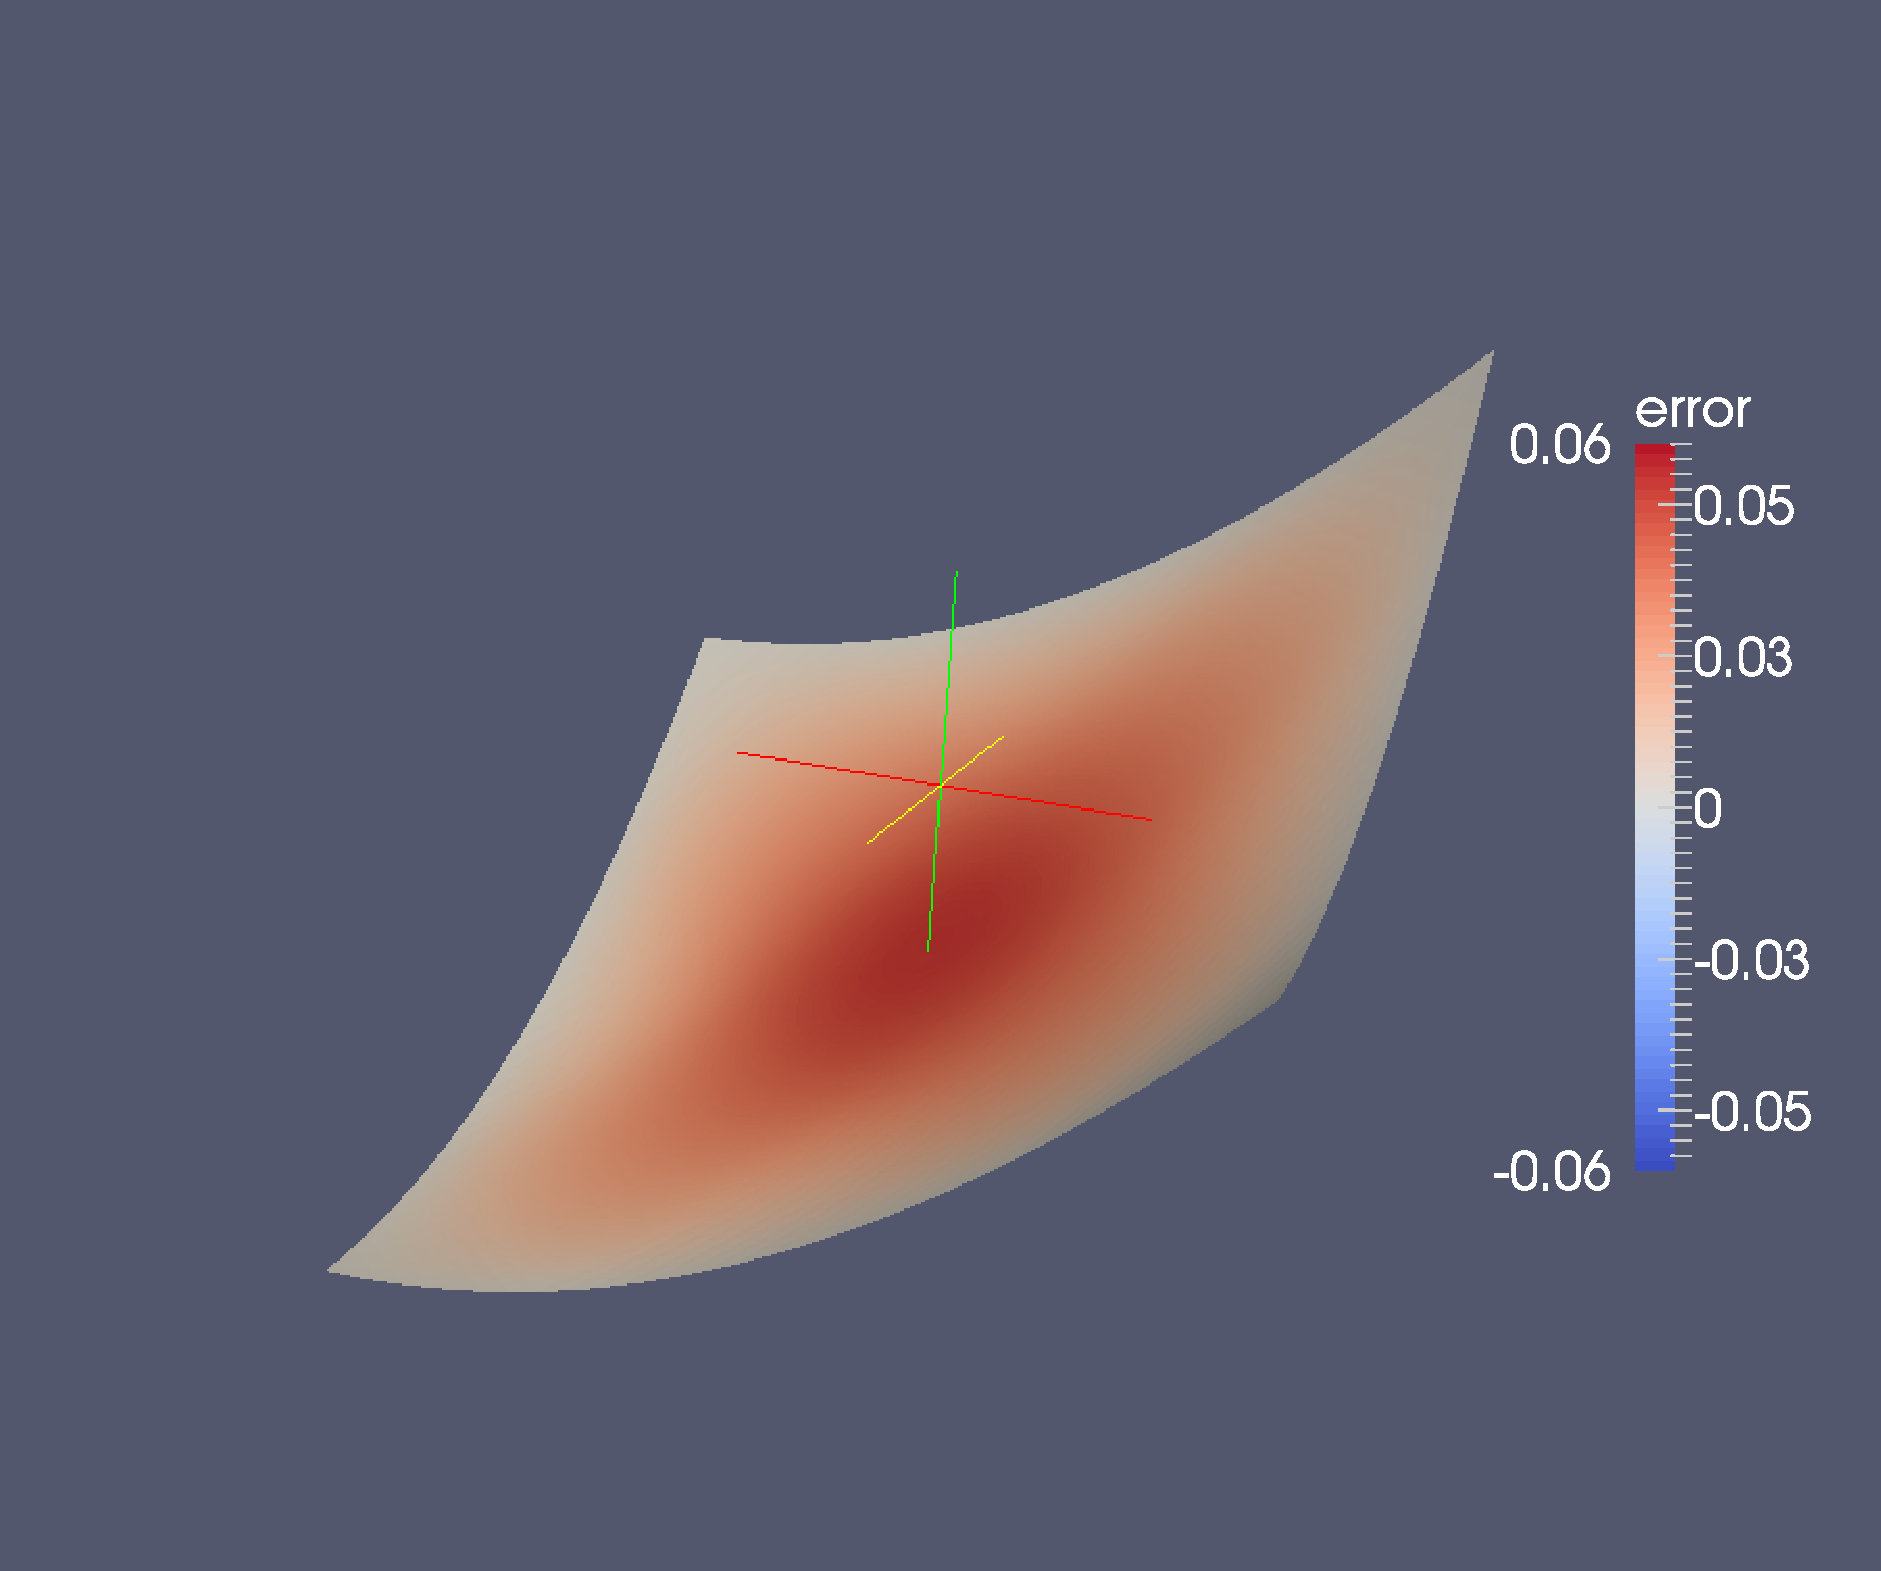
\includegraphics[width=1.\textwidth]{../Arbeit/plots/with_penalty_it22.pdf}
		\caption{Solution after 23 steps}
	\end{subfigure}
	~
	\begin{subfigure}[b]{.45\textwidth}
		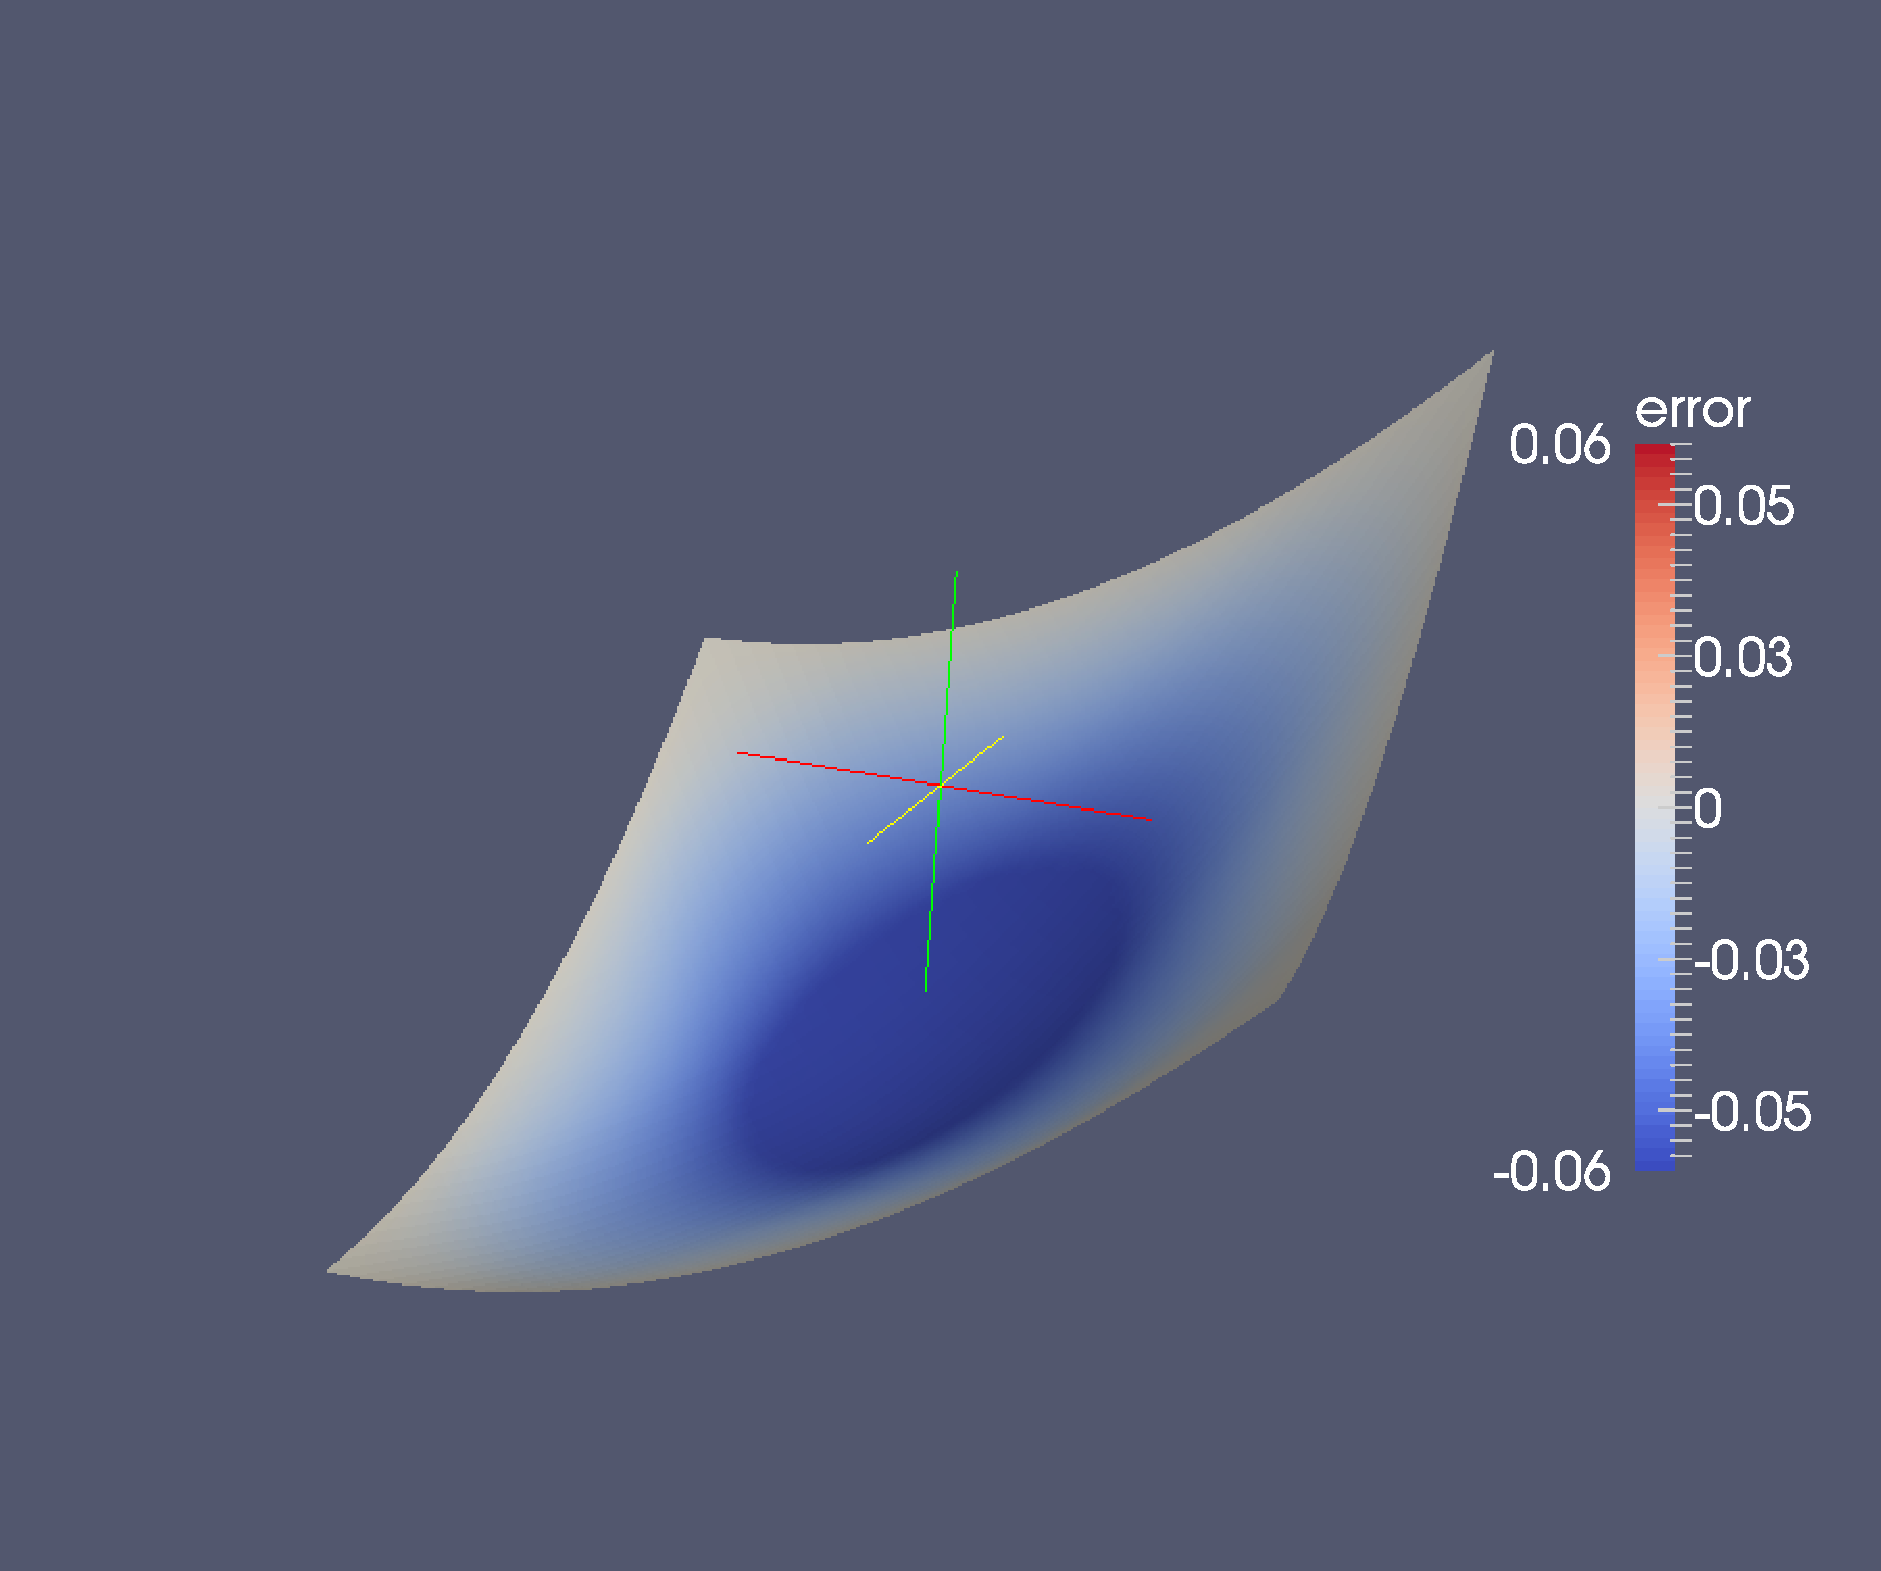
\includegraphics[width=1.\textwidth]{../Arbeit/plots/with_penalty_it23.pdf}
		\caption{Solution after 24 steps}
	\end{subfigure}
	\caption{Die Lösung zweier aufeinander folgender Iterationen}
	\end{figure}
\end{frame}

\begin{frame}{Damping of the Picard iteration}
	\begin{figure}[H]
		\centering
		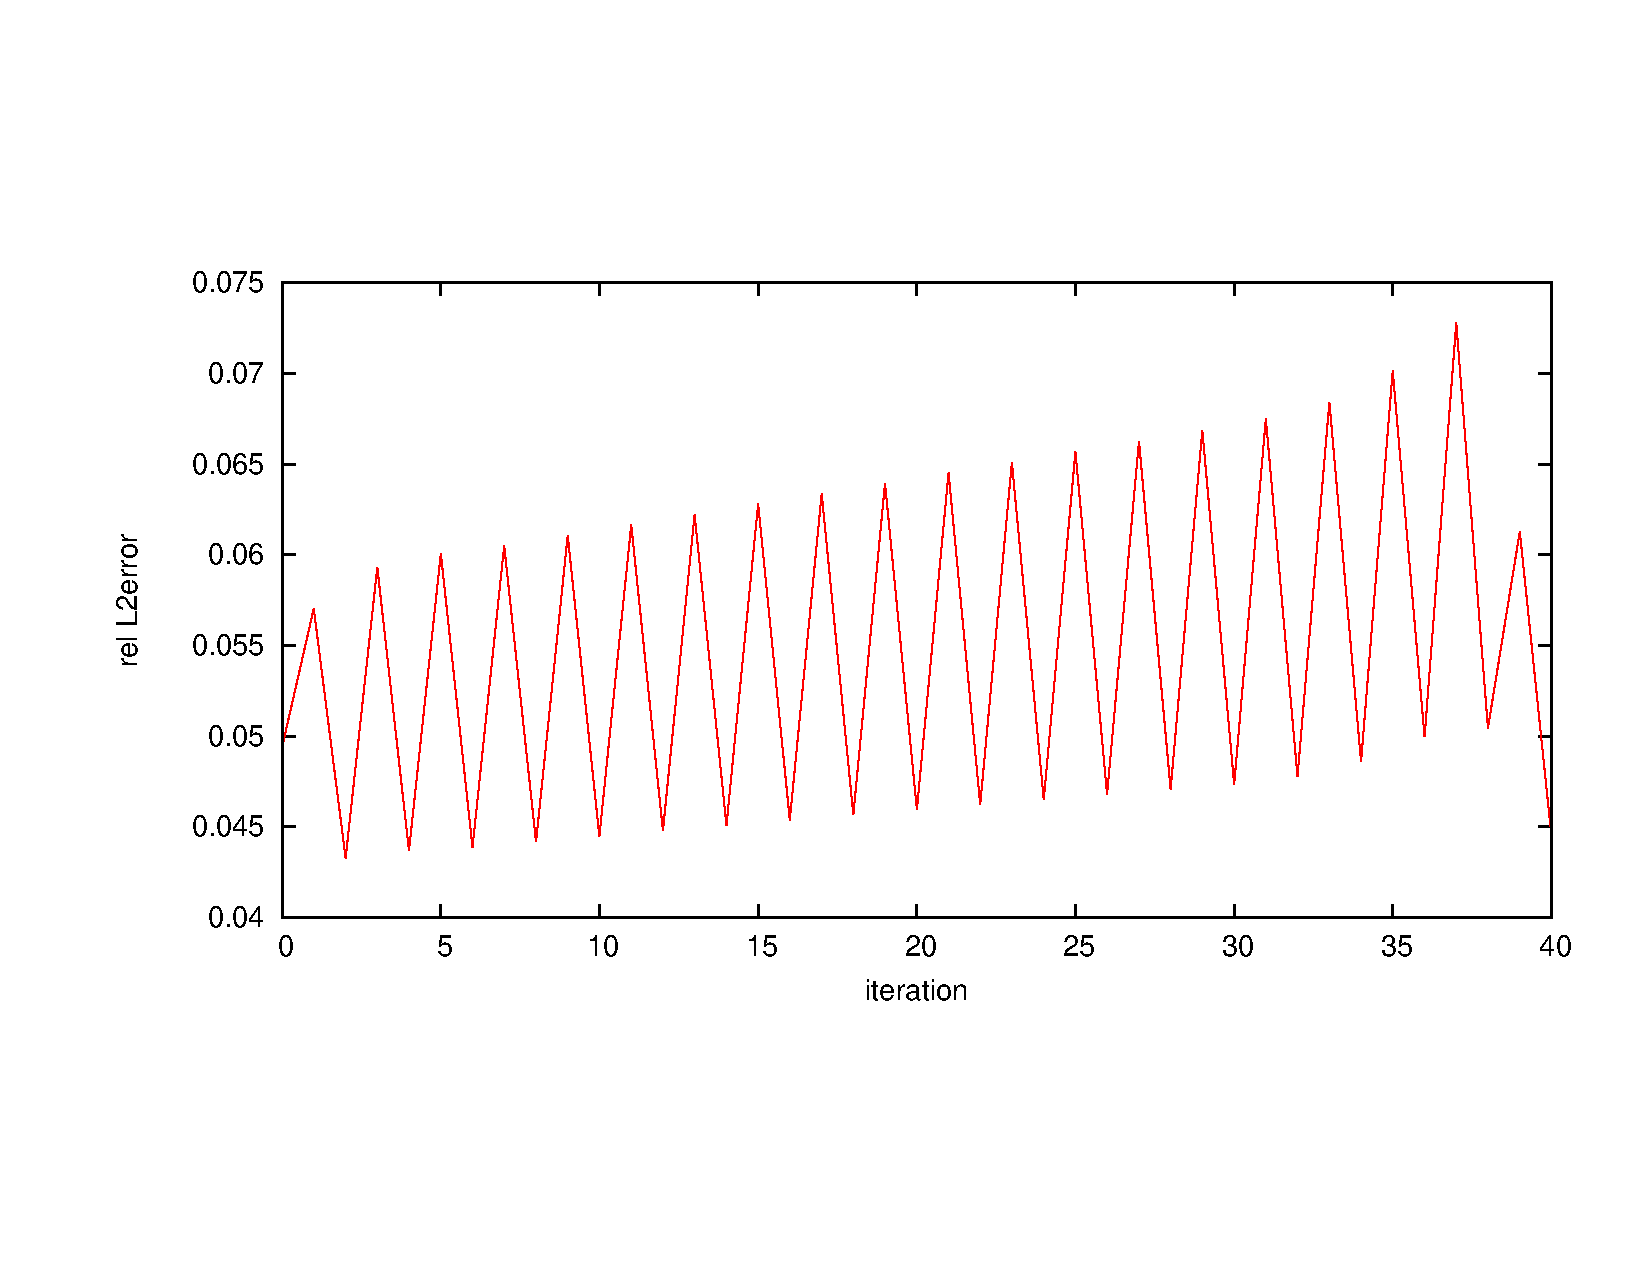
\includegraphics[trim = 2cm 4cm 1cm 4cm, height = 0.6\textheight]{../Arbeit/plots/oscillation.pdf}
		\caption{Relative $L^2$ error on a grid with $h=\frac 1 4$ and gradient penalty}
		\label{fig: oscillation}
	\end{figure}
	\pause
	\vspace{-0.5cm}
	$\Rightarrow$ Convex combination $ \alpha u_h^{i+1} + (1- \alpha) u_h^i$ for $\alpha \in (0,1)$
\end{frame}


\begin{frame}{Well-posedness of SIPG formulation}
\begin{itemize}
	\item The ellipticity constant of the SIPG bilinear form is only positive for $\sigma > \sigma^*$. 
	\pause
	
	\item $\sigma^*$ depends on $1/\lambda(\cofHess u)$, where  $\lambda(A)$ denotes the smallest eigenvalue of $A$.
\end{itemize}
	\pause
	$\Rightarrow$ scale $\sigma$ by $\frac 1 {\lambda^*}$ where $\lambda^*$ is an approximation of the smallest eigenvalue.\pause We choose
	
	\begin{block}{Approximation of $\lambda$}
	\[
		\lambda^* = \min_{q \in Q} \lambda(\cofHess {u_h(q)}),
	\]
	where $Q$ are the quadrature points.
	\end{block} 
	
\end{frame}

\begin{frame}{Well-posedness of SIPG formulation}
\begin{itemize}
	\item For ellipticity of the SIPG bilinear form we need $\mycof {D^2_h u_h}$ to be positive definite.\\
	\pause
	\item Bound ellipticity constant from below with a constant
\end{itemize}
	\pause
	\begin{block}{Modified Cofactor Matrix}
		\[ 
			\mycofMod {D^2_h u_h} = \begin{cases}
			\mycof {D^2_h u_h} & \lambda \geq \varepsilon	\\
			\mycof {D^2_h u_h}+ (-\lambda+\varepsilon) Id%\begin{pmatrix} -\lambda+\varepsilon & 0 \\ 0 & -\lambda+\varepsilon \end{pmatrix} 
			& else
			\end{cases}
		\]
	\end{block}
	\pause
	\[
		\mycof {D^2_h u_h} \text{ pos. def.} \Leftrightarrow \hess u \text{ pos. def.} \pause \Leftrightarrow u_h \text{ is convex}
	\]
	
	
\end{frame}



\begin{frame}{Convexification of intermediate solutions}
\begin{itemize}
	\item \MA equation in general does not posses a unique solution
	\item often (unique) convex solution required
\end{itemize} 
\pause
	$\Rightarrow$ convexify the solution after every step
\begin{itemize}
\pause
	\item connection between convexity and B\'ezier polynomials
	\item convexification is not simple
	\item discussion in numerical results
\end{itemize} 
\end{frame}

%\begin{frame}{Convexification Approach of Schumaker and Speleers{, \cite{SS2014}}}
%	Given the solution of the generalised Poisson problem $u^{gp}_h$ we seek for a convex spline minimising the error at the B\'ezier control points, i.e. 
%\begin{block}{Quadratic Program for Convexification}
%Find the B\'ezier coefficients $c$ minimising
%	\begin{align*}
%			\lVert A c - b \rVert_2, \qquad \text{ such that } Cc \geq 0. %\label{eq: convex lsq}
%	\end{align*}
%\end{block}
%\begin{itemize}
%	\item $A$ is the matrix evaluating the piecewise polynomial at the B\'ezier control points
%	\item $b$ are the function values of $u^{gp}_h$ at the B\'ezier control points
%	\item  $C$ is the matrix containing the conditions ensuring convexity on the whole domain
%\end{itemize}
%
%\end{frame}


%\subsection{Algorithm for the Picard Iteration}

\begin{frame}
\begin{algorithm}[H]
\begin{algorithmic}
\Require triangulation \triang, desired mesh width $H$, maximal number of intermediate steps $i_{max}$
\State $u_{0}\gets $ solution of  $
	\triangle u = \sqrt{2f} \text{ in } \Omega $ with $
	u = g \text{ on }\partial \Omega$ %\Comment initialisation
\While {$h < H$}
	\For {$i$ from 1 to $i_{max}$}
		\State $\sigma \gets \sigma /\lambda(\hess{u_h^{i-1}}) $
		\State $u_i \gets$ sol of generalised Poisson problem w. modified cofactor matrix
		\State (convexify)
		\State $u_i \gets \alpha u_{i-1} + (1-\alpha)u_i $ \Comment convex combination
	\EndFor
	\State $h, \triang, u_{0} \gets h/2, \triangFine, u_{i_{max}}$
\EndWhile
\end{algorithmic}
\caption{Picard Iteration Algorithm to Solve the MA Equation}
\label{alg: final}
\end{algorithm}
\end{frame}


\section{Numerical Results}

\subsection{Implementation}
\begin{frame}{Implementation}
	\begin{itemize}
		\item implemented in C++
		\item linear system solved directly by a cholesky decomposition
		\item convexification via a quadratic program (c.f. {\cite{SS2014}}) solved by the library IPOPT
		\item 15 steps on each grid before refinement
		\item uniform standard grid refinement
	\end{itemize}
\end{frame}

\subsection{Results with Convexification}
\begin{frame}{Smooth test problem}
\vspace{-0.5cm}
\[
	u=\exp( \lVert x \rVert_2^2  /2) 
	\text { and } 
	f = (1 + \lVert x \rVert_2^2) \exp( \lVert x \rVert^2).
\]
\vspace{-0.75cm}
\begin{figure}[H]
\centering
	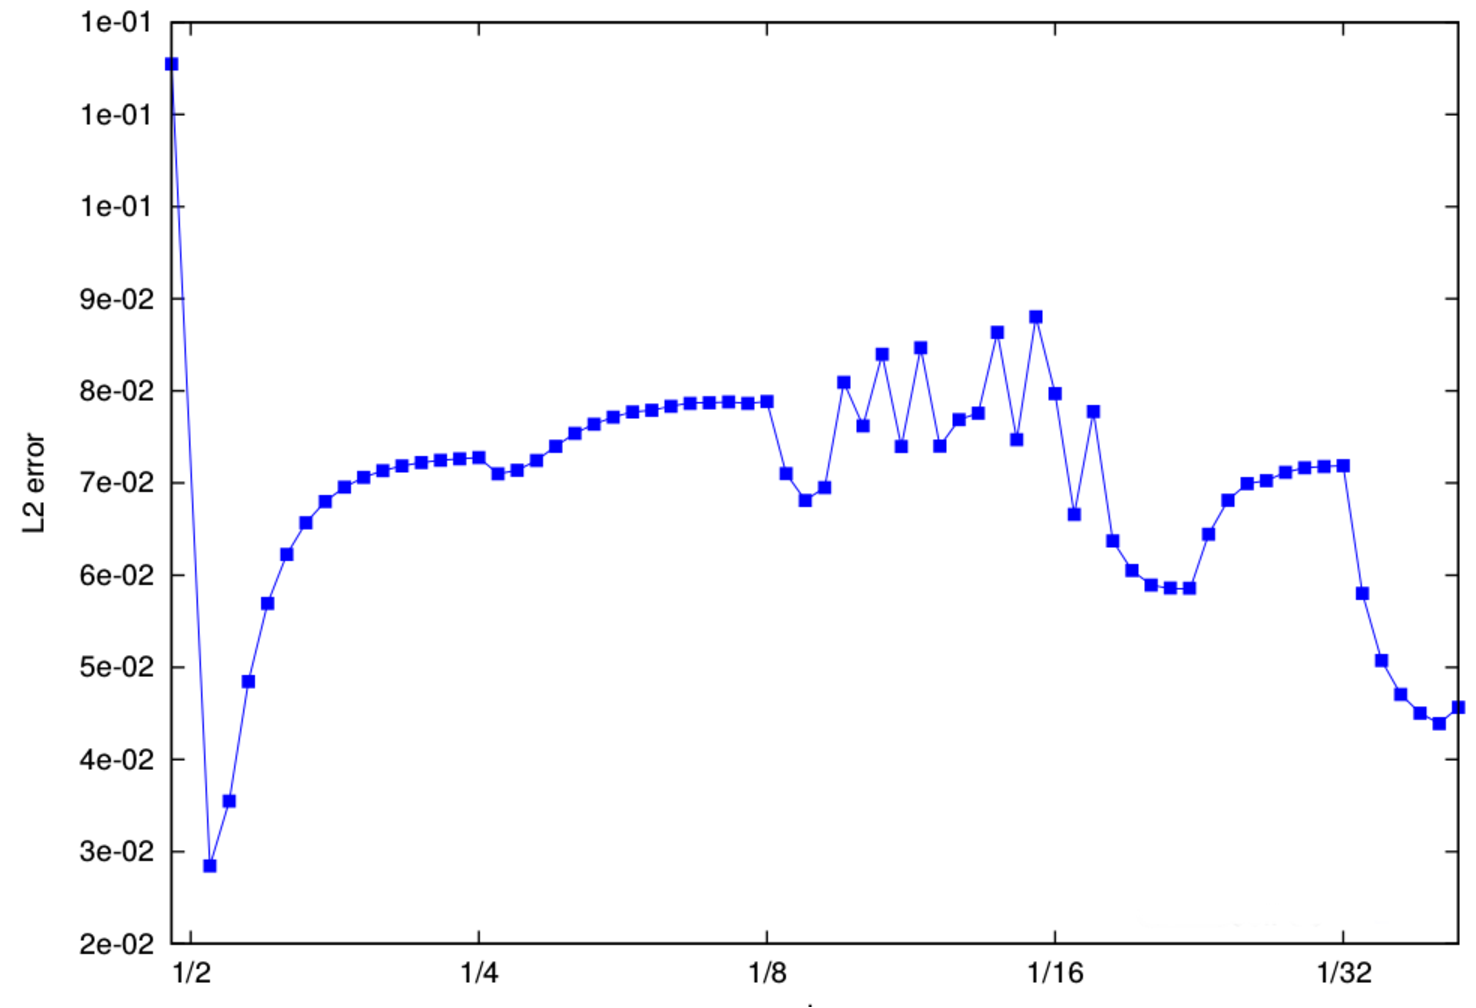
\includegraphics[height=0.75\textheight]{MA1_convexify_cropped.pdf}
%	\caption{$L^2$ errors for Test \ref{test smooth} and additional convexification}
\end{figure}
\end{frame}

\begin{frame}{Impact of convexifaction}
Comparison of $L^2$ errors before and after convexification
\vspace{-0.75cm}
\begin{figure}[H]
	\centering
	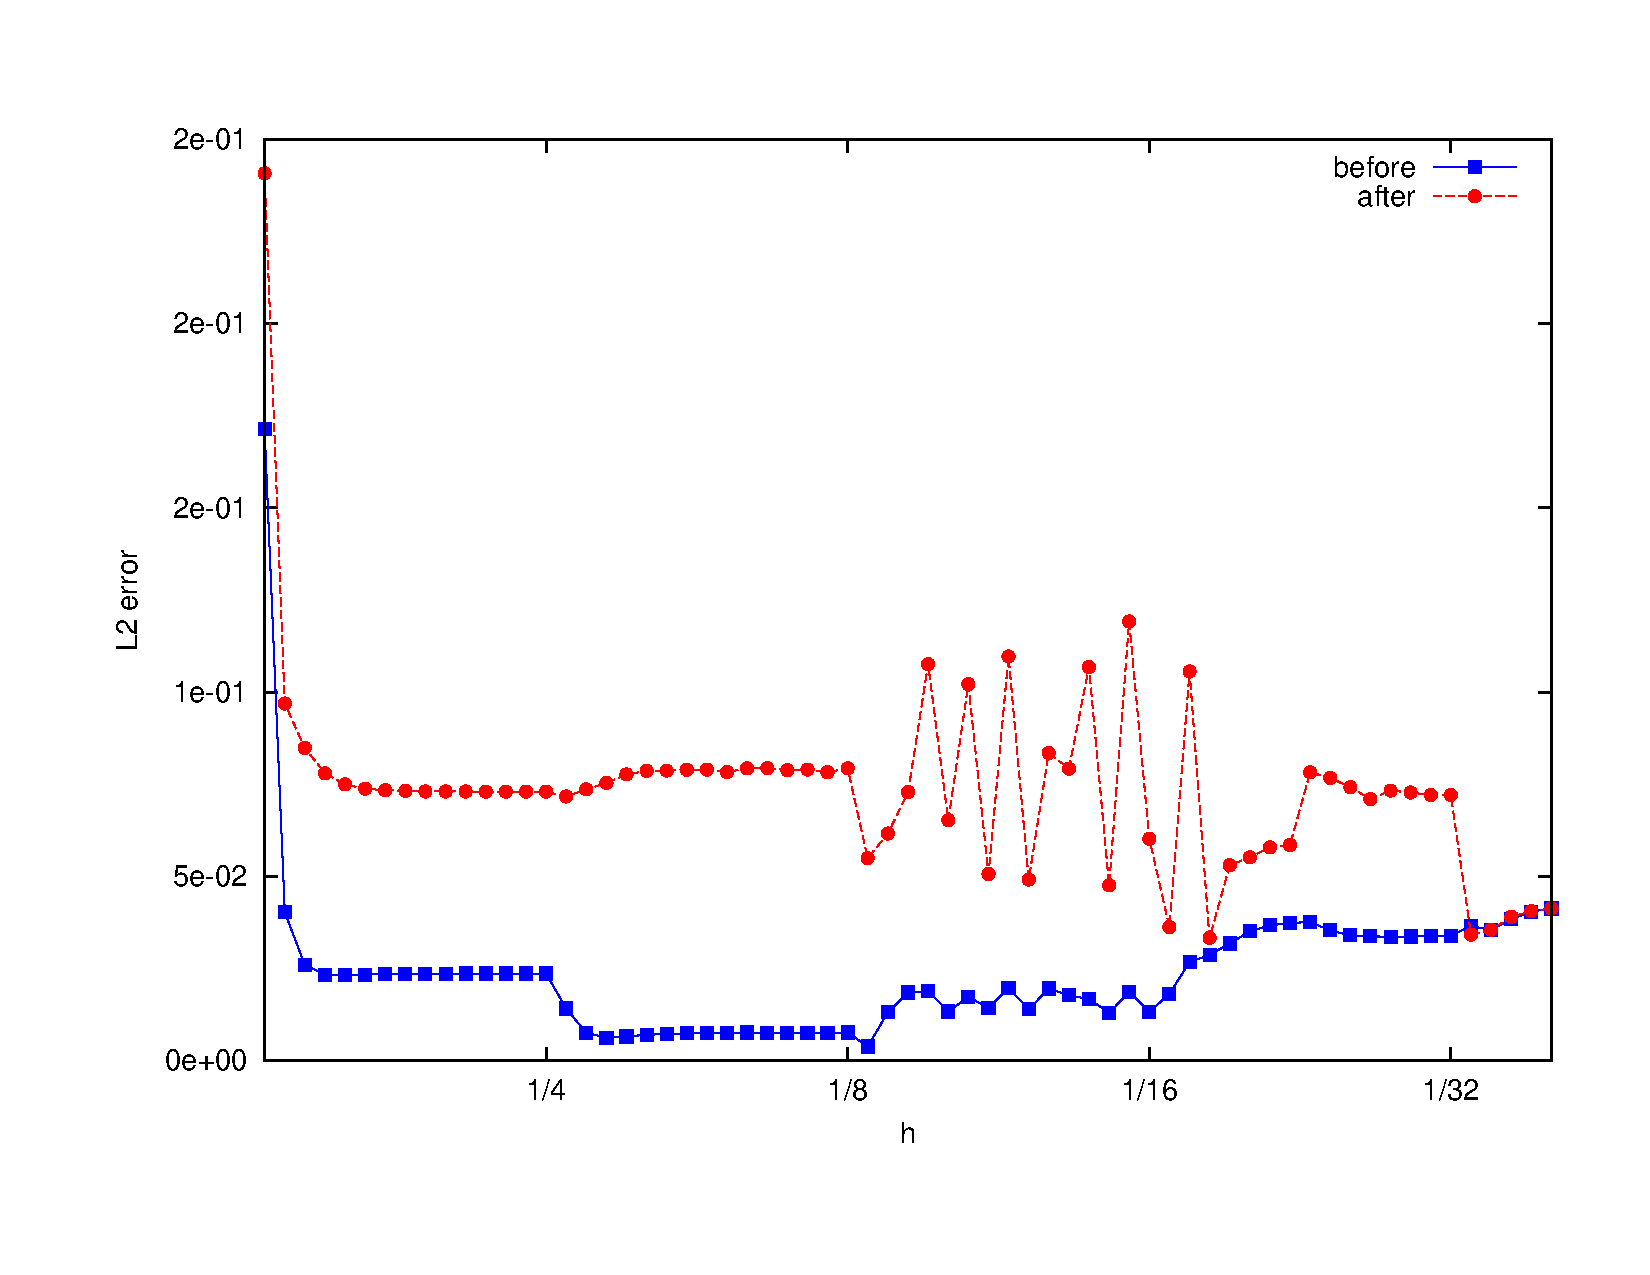
\includegraphics[height=0.95\textheight]{../Arbeit/plots/MA1_convexComp.pdf}
\end{figure}
\end{frame}

\subsection{Results without Convexification}
\begin{frame}{Smooth test problem without convexification}
%\end{block}
\vspace{-0.75cm}
	\begin{figure}[H]
	\centering
	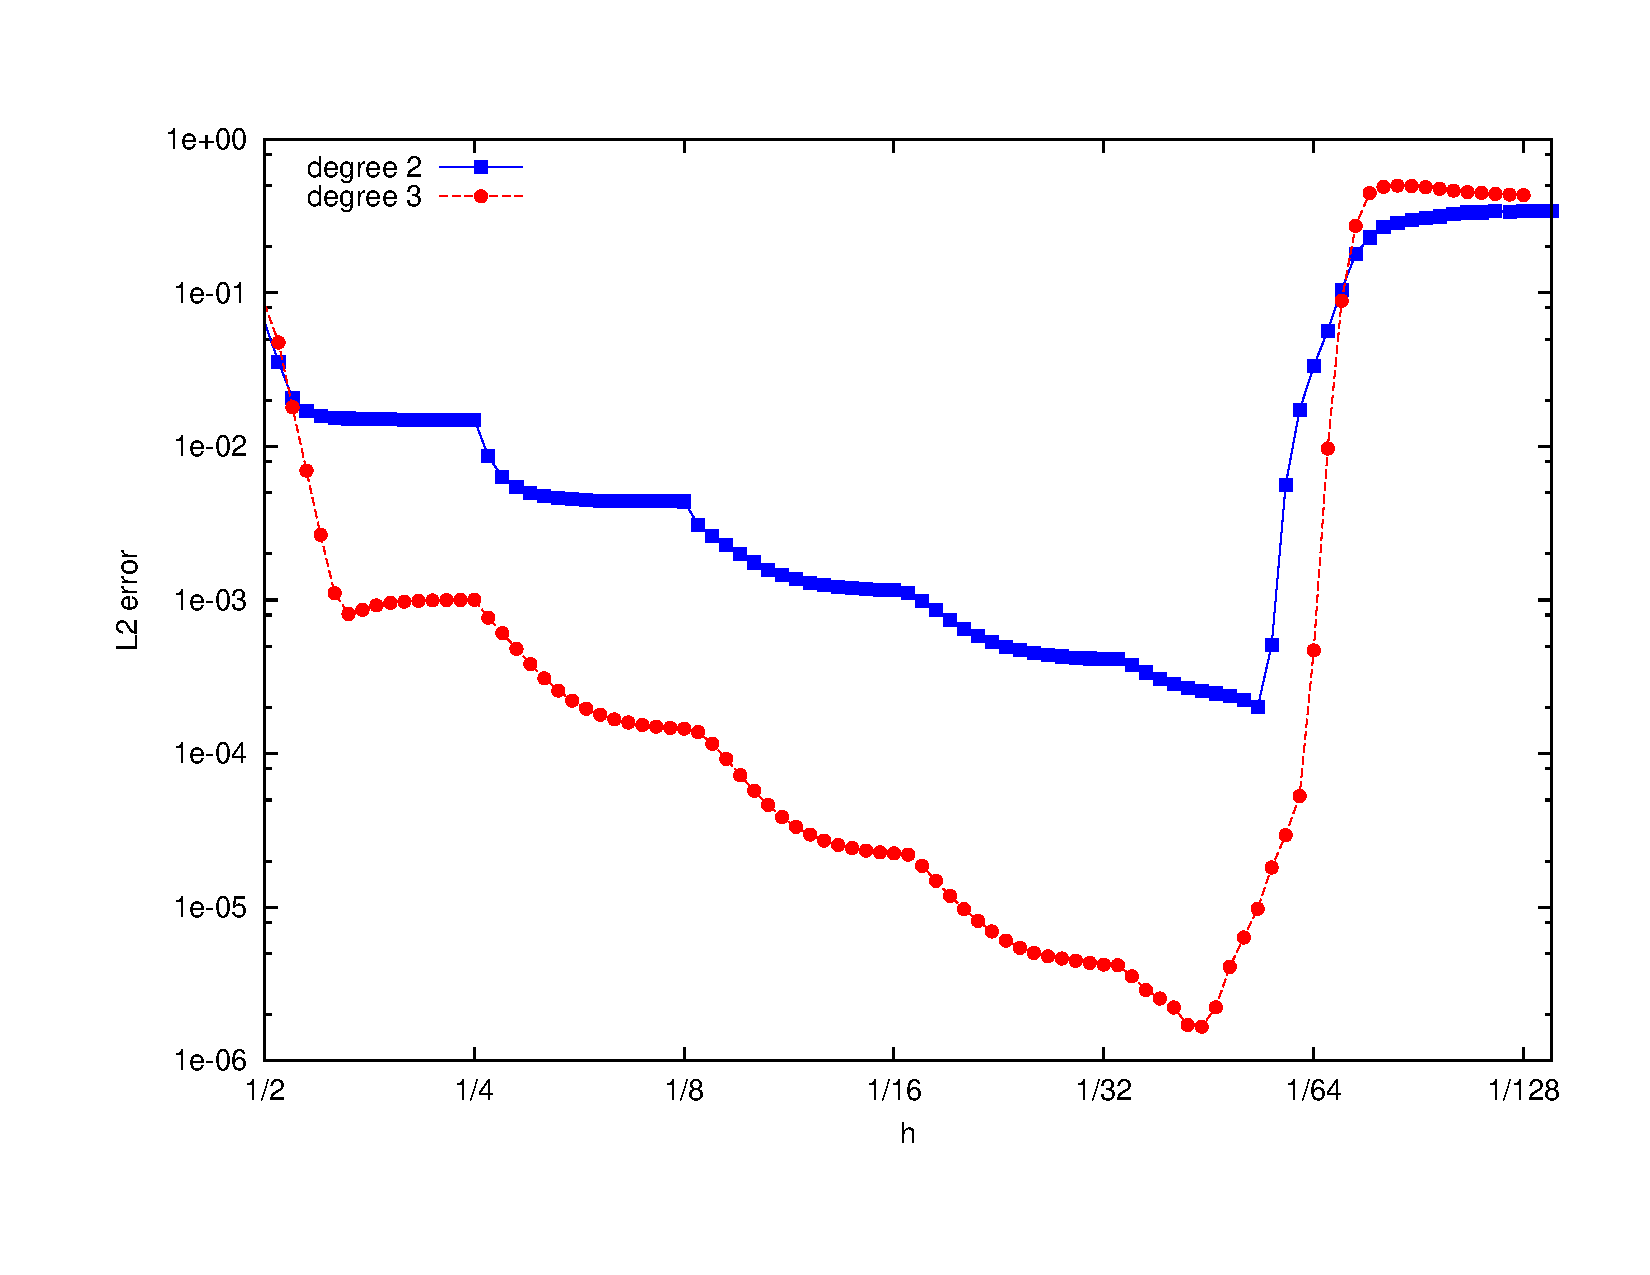
\includegraphics[ %trim = 3cm 4cm 0cm 2cm,
	width=\textwidth]{../Arbeit/plots/MA1.pdf}
%		\caption{$L^2$ error with grad penalty}
	\end{figure}
\end{frame}

\begin{frame}{Penalty parameter $\sigma^G$}
$L^2$ errors for different choices of $\sigma^G$
\vspace{-0.75cm}
\begin{figure}[H]
	\centering
	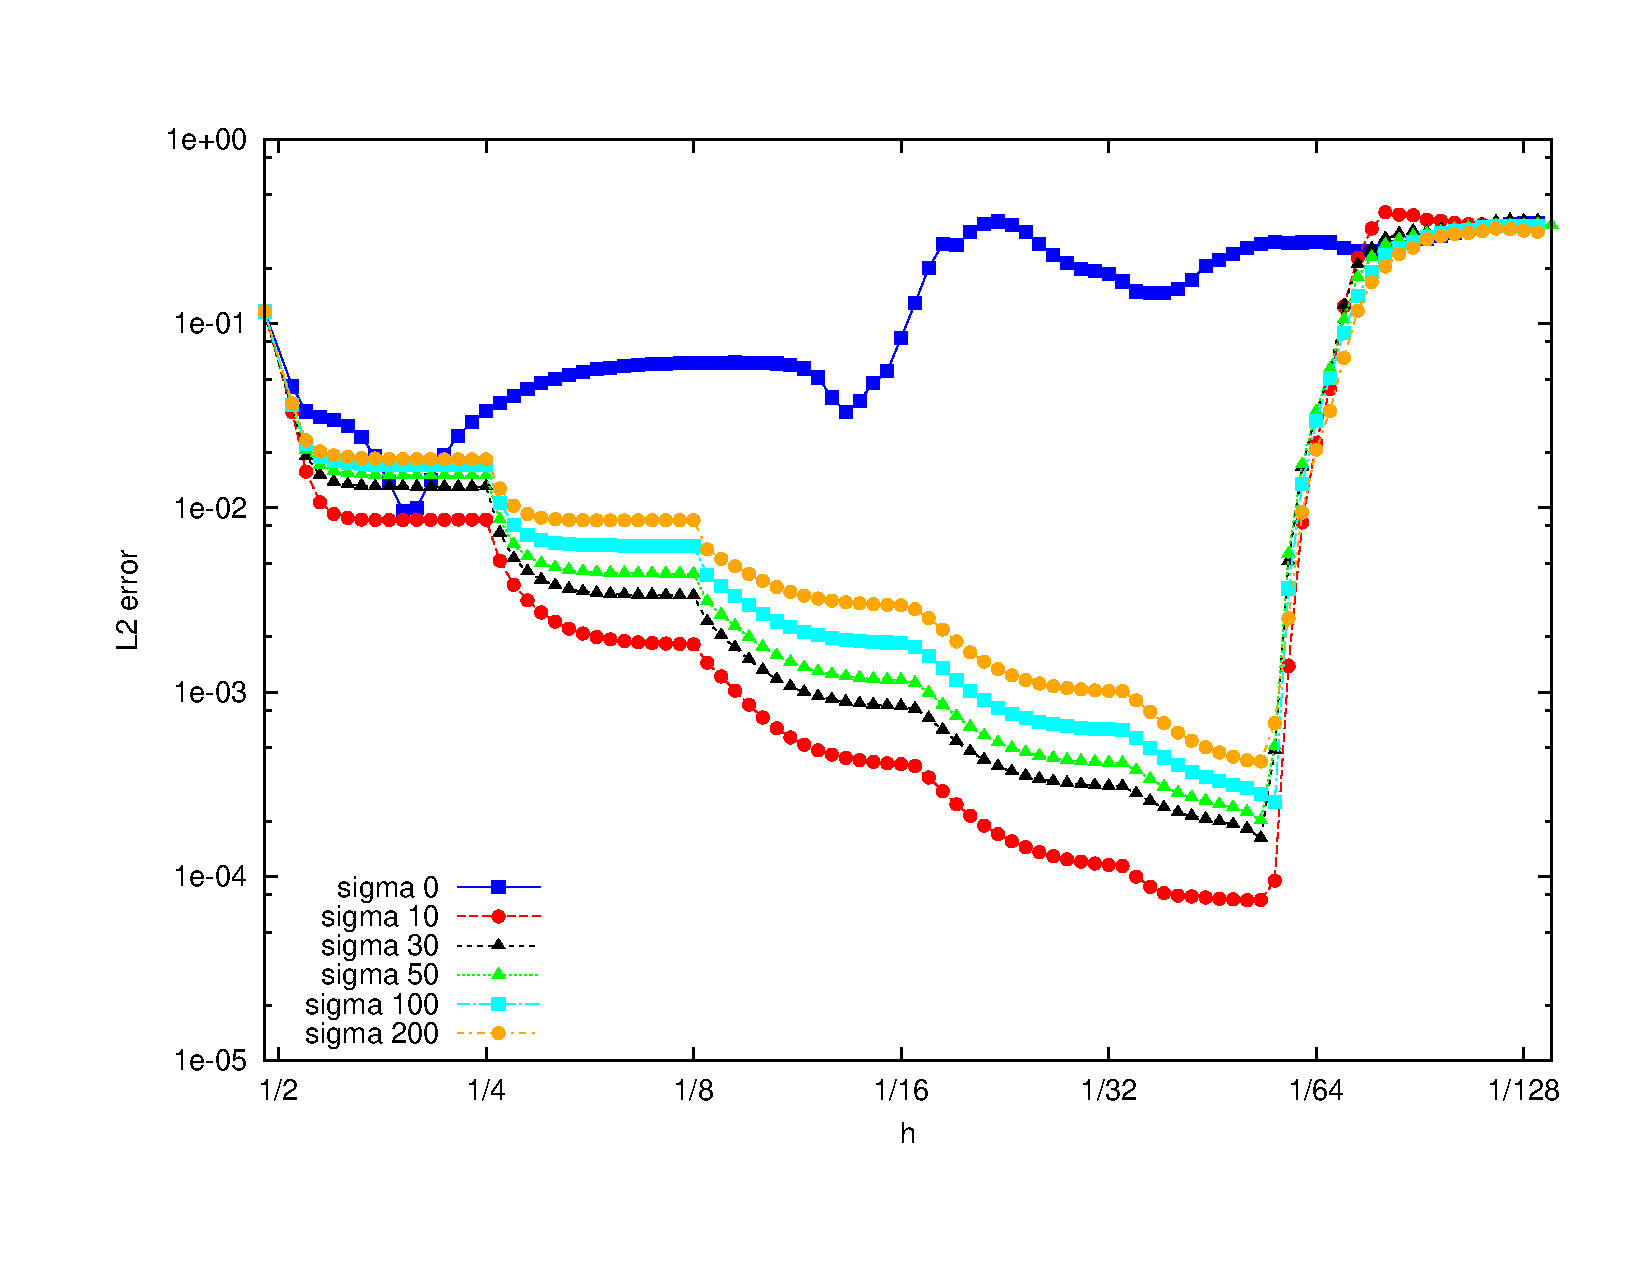
\includegraphics[height=0.95\textheight]{../Arbeit/plots/MA1_deg2_sigma.pdf}\end{figure}
\end{frame}

\begin{frame}{Convex combination with parameter $\alpha$}
$L^2$ errors for different choices of $\alpha$
\vspace{-0.75cm}
\begin{figure}[H]
	\centering
	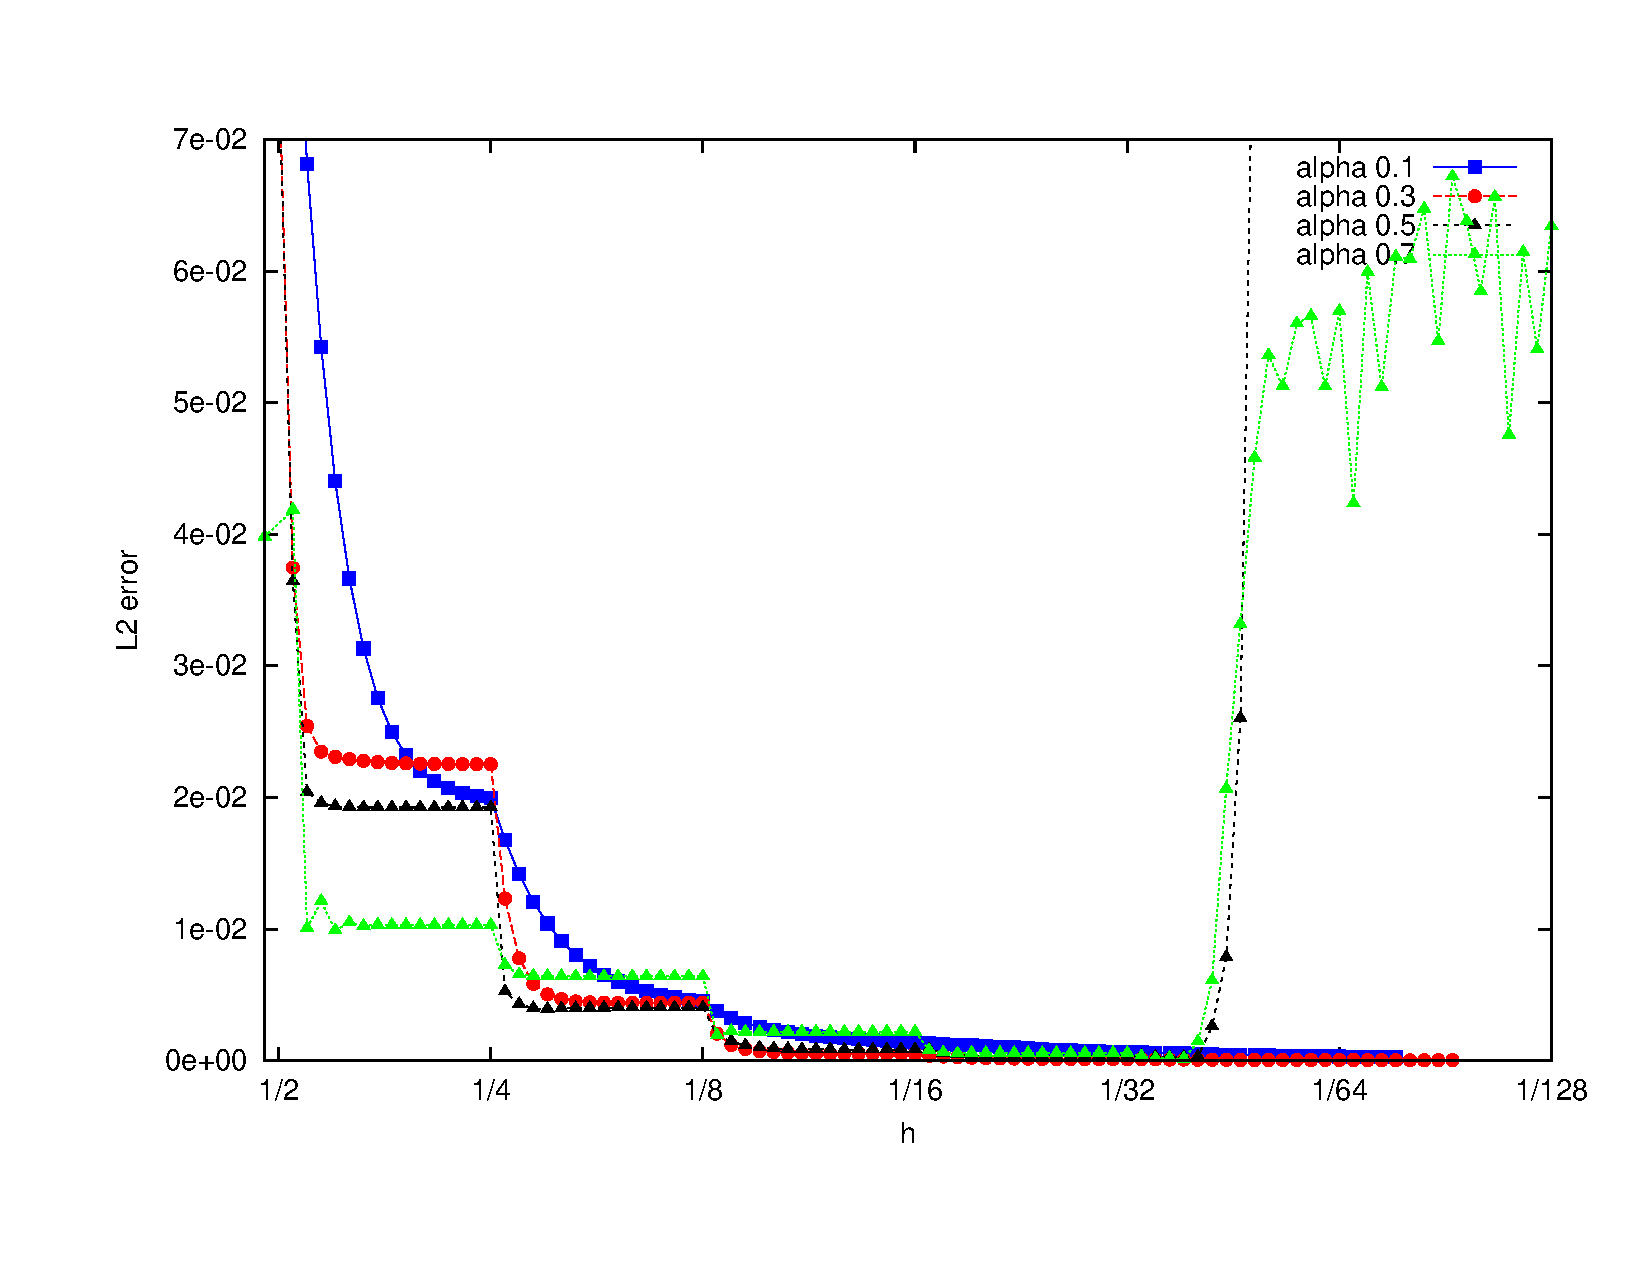
\includegraphics[height=0.95\textheight]{../Arbeit/plots/MA1_deg2_alpha.pdf}\end{figure}
\end{frame}

\begin{frame}{$C^1$ test problem}
\vspace{-0.5cm}
\[
	u=\frac 1 2 \left( \max 0 {\lVert x - x_0 \rVert_2-0.2 }  \right)^2 
	\text { and } 
	f = \max 0 {1-\frac {0.2} {\lVert x - x_0 \rVert_2} }.
\]
\vspace{-0.75cm}
\begin{figure}[H]
\centering
	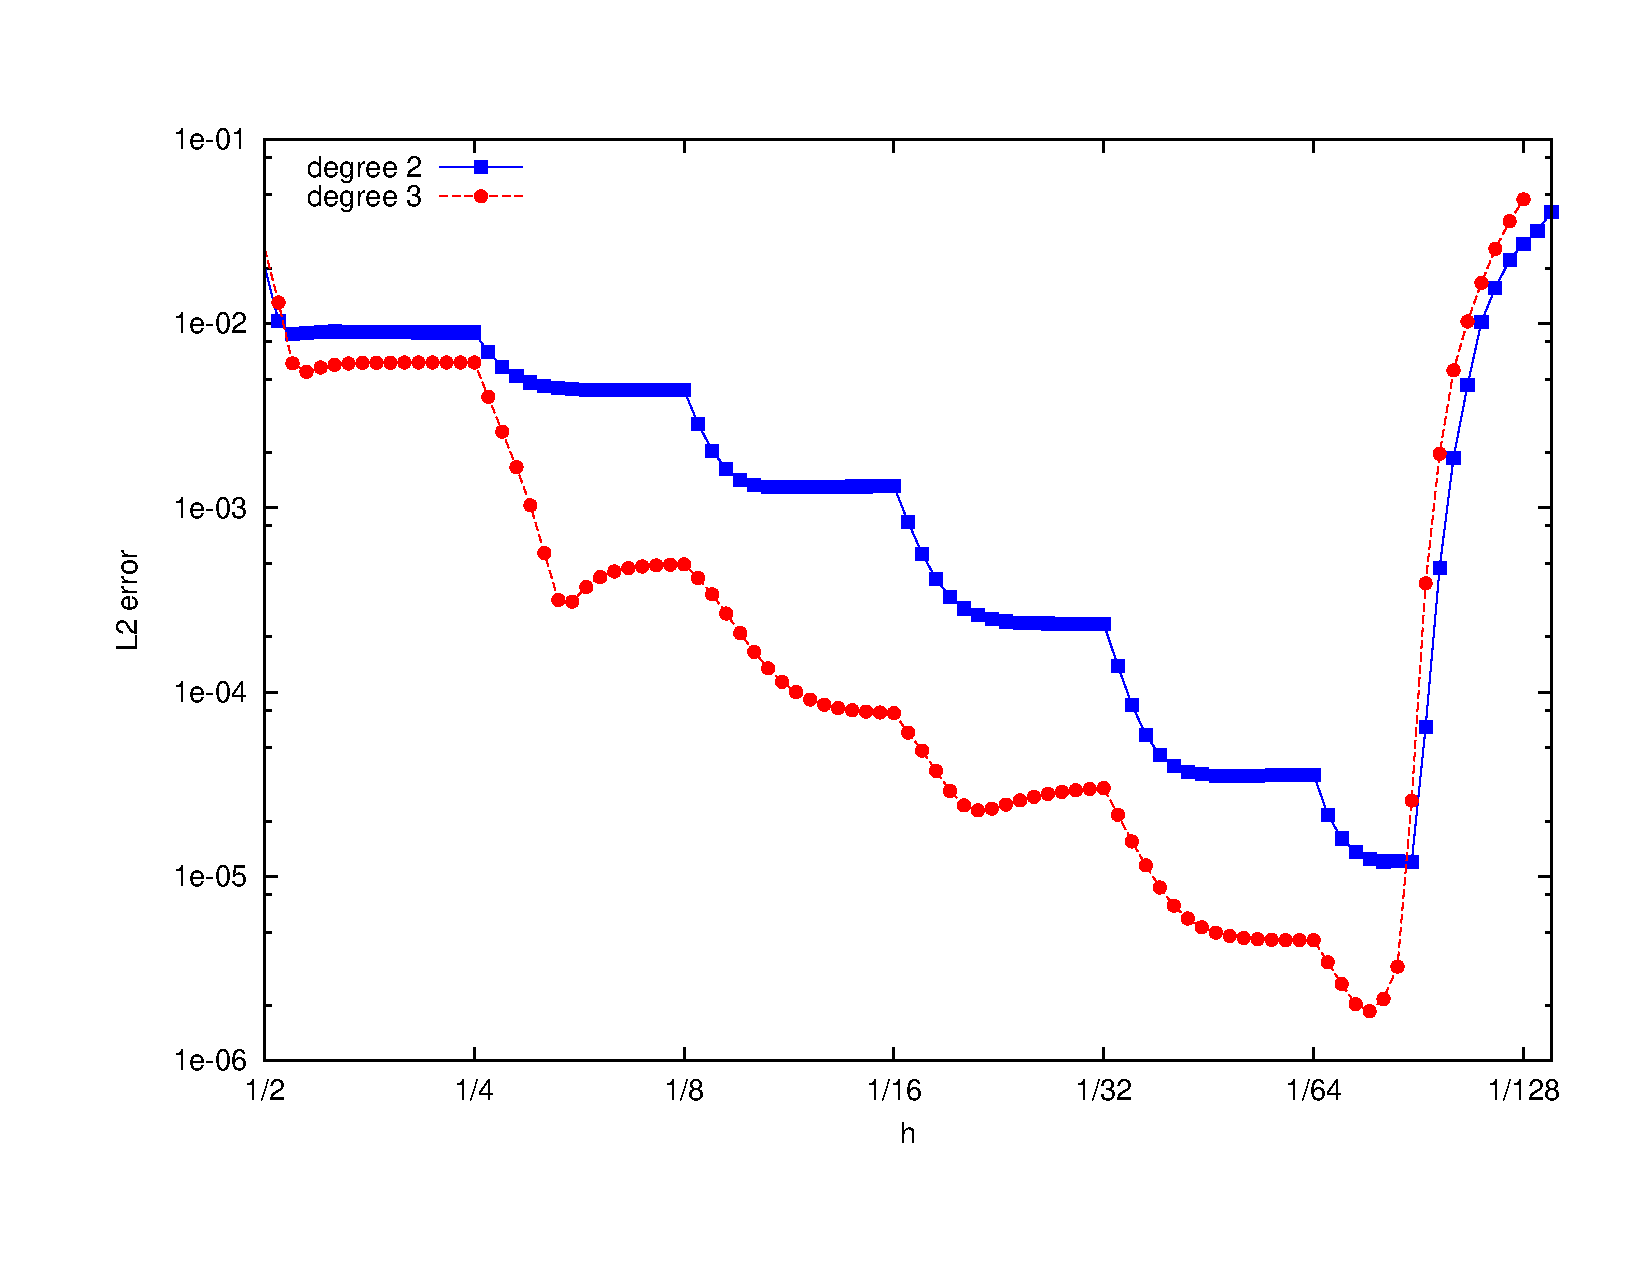
\includegraphics[height=0.85\textheight]{../Arbeit/plots/MA2.pdf}
%	\caption{$L^2$ errors for Test \ref{test smooth} and additional convexification}
\end{figure}
\end{frame}

\begin{frame}{Singular test problem}
\vspace{-0.5cm}
\[
	u = - \sqrt{ 2-  \lVert x \rVert_2^2}
	\text { and } 
	f = 2\left( 2-  \lVert x \rVert_2^2 \right)^{-2}
\]
\vspace{-0.75cm}
\begin{figure}[H]
\centering
	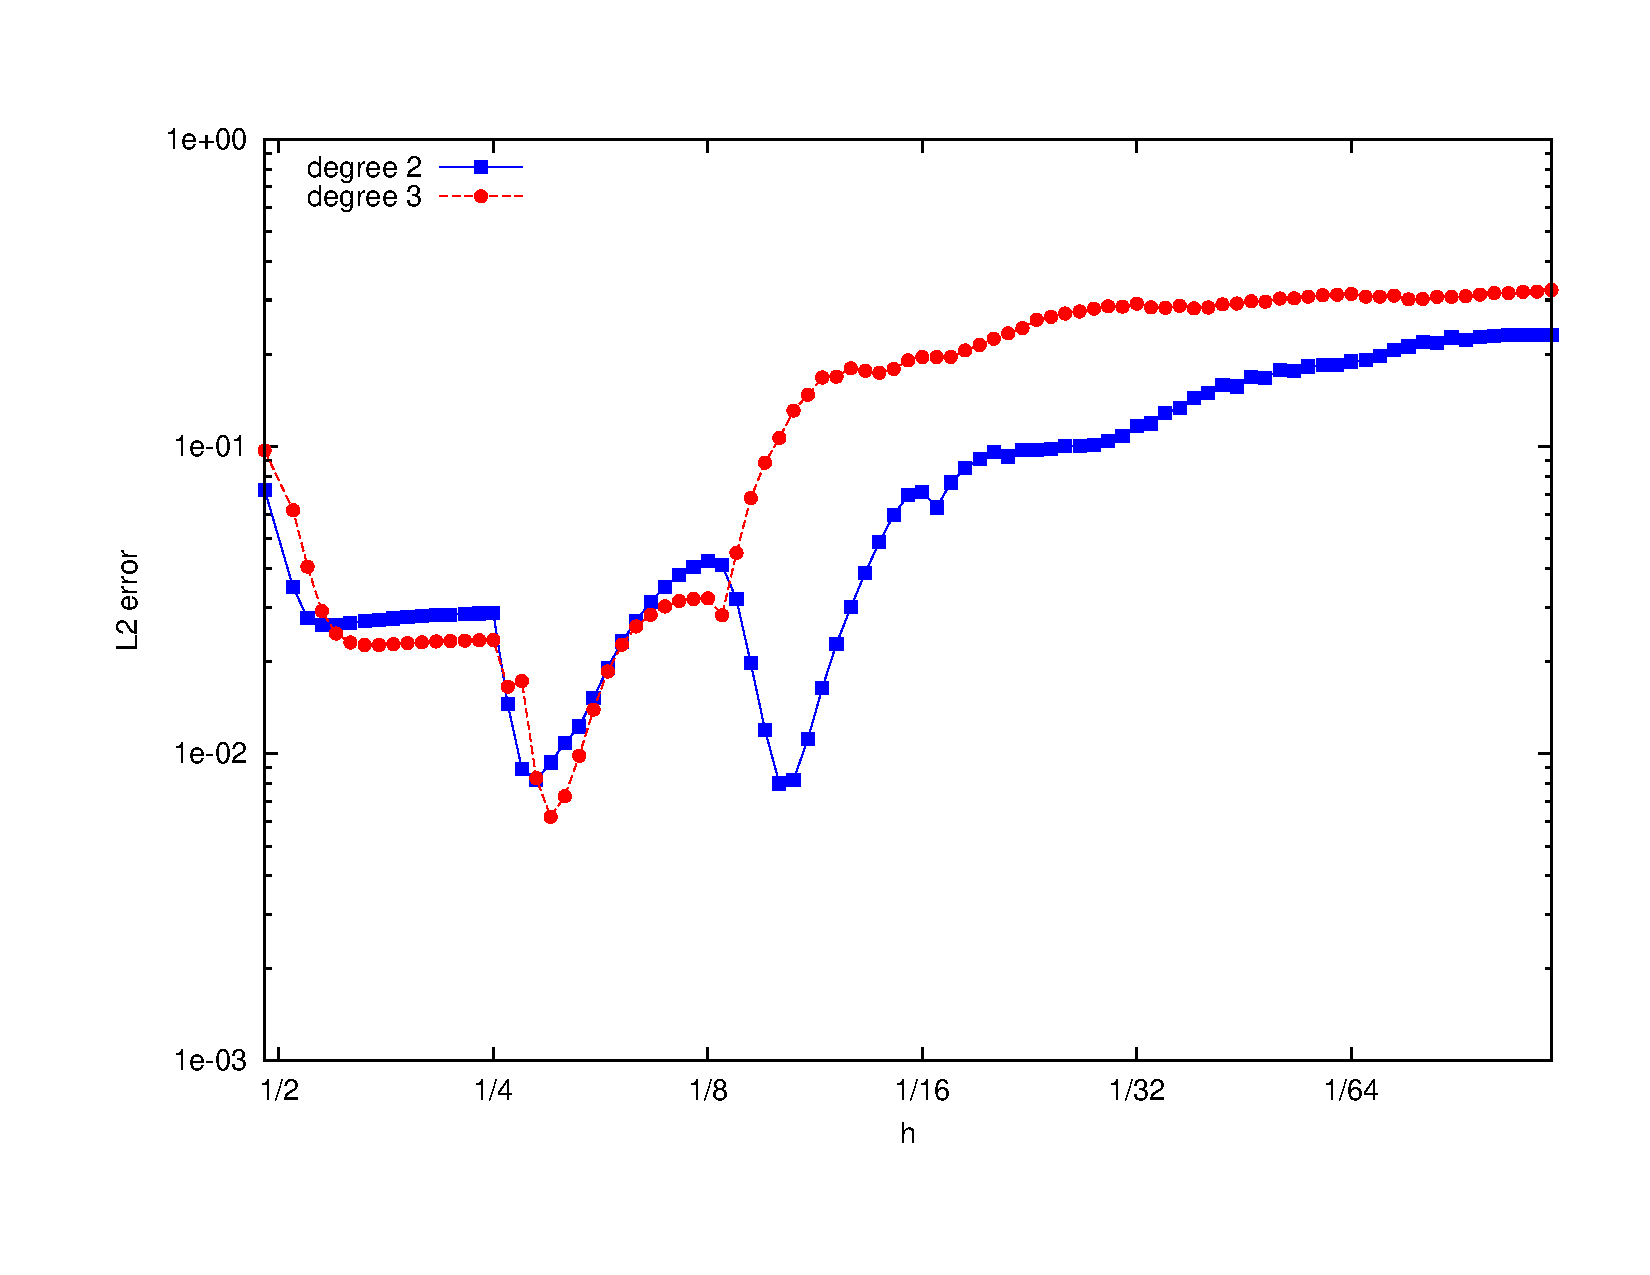
\includegraphics[height=0.85\textheight]{../Arbeit/plots/MA3.pdf}
%	\caption{$L^2$ errors for Test \ref{test smooth} and additional convexification}
\end{figure}
\end{frame}


\section{Conclusion and Perspective}

\begin{frame}{Conclusion}
	\begin{itemize}
		\item reviewed current DG methods
		\item derived a new DG method using Picard linearisation
		\item explored several improvements of the Picard DG method
		\item the Picard type iteration converges on coarse grids, but is unstable on finer grids
		\item current DG methods are applicable for problems with smooth solutions, but have problems or even fail on singular problems
	\end{itemize}
\end{frame}

%\subsection{Conclusion}
	
\begin{frame}{Perspective}
	\begin{itemize}
		\item investigate if decoupled PDE has more solutions than the solution $v=w$
		\item implemented convexification not useful, may only convexify on finer grids
		\item analysis of the impact of the gradient penalty term
		\item apply theory developed for Picard linearisations of convection terms
		\item extension to right-hand sides depending on $u$ and $\nabla u$ and more complicated left-hand sides
		\item three-dimensional case
	\end{itemize}
\end{frame}


\begin{frame}[allowframebreaks]{References}
\putbib[../Arbeit/my_additional_bibliography.bib]
\end{frame}
\end{bibunit}


\end{document}